%%%%%%%%%%%%%%%%%%%%%%%%%%%%%%%%%%%%%%%%%%%%%%%%%%%%%%%%%%%%%%%%%%%%%
%% This is a "template" model document for submission to the
%% American Chemical Society (ACS).
%%
%% The guidance here contains information about how you may wish to
%% modify it to match the requirements of various ACS journals. The
%% ACS do *not* typeset accepted articles using LaTeX, so there is
%% no specific class required.
%%
%% This template deliberately does *not* seek to reproduce
%% the layout of the typeset journal: this is explicitly not
%% required by the ACS for LaTeX submissions.
%%
%% Please report any issues with the template at
%% https://github.com/josephwright/acs-template/issues
%%
%% Released under the Creative Commons 0 license
%% https://creativecommons.org/public-domain/cc0/
%% 
%% Copyight (c) 2025 Joseph Wright
%%%%%%%%%%%%%%%%%%%%%%%%%%%%%%%%%%%%%%%%%%%%%%%%%%%%%%%%%%%%%%%%%%%%%
\documentclass[letterpaper]{article}

%%%%%%%%%%%%%%%%%%%%%%%%%%%%%%%%%%%%%%%%%%%%%%%%%%%%%%%%%%%%%%%%%%%%%
%% Font setup - delete if you are using LuaLaTeX
%%%%%%%%%%%%%%%%%%%%%%%%%%%%%%%%%%%%%%%%%%%%%%%%%%%%%%%%%%%%%%%%%%%%%
\usepackage[T1]{fontenc}

%%%%%%%%%%%%%%%%%%%%%%%%%%%%%%%%%%%%%%%%%%%%%%%%%%%%%%%%%%%%%%%%%%%%%
%% Adjust the margins and allow for line spacing
%%%%%%%%%%%%%%%%%%%%%%%%%%%%%%%%%%%%%%%%%%%%%%%%%%%%%%%%%%%%%%%%%%%%%
\usepackage{geometry}
\geometry{margin = 1in}
\usepackage{setspace}

%%%%%%%%%%%%%%%%%%%%%%%%%%%%%%%%%%%%%%%%%%%%%%%%%%%%%%%%%%%%%%%%%%%%%
%% Reference support
%%
%% The recommended method for producing the reference section is
%% to use biblatex. If you wish to use a classical BibTeX
%% approach, this is easiest to achieve using the achemso package.
%% In that case, you should remove the biblatex lines.
%%%%%%%%%%%%%%%%%%%%%%%%%%%%%%%%%%%%%%%%%%%%%%%%%%%%%%%%%%%%%%%%%%%%%
% You can adjust the printing of DOI, article title, etc. using
% package options, e.g. "doi = true"; see the biblatex manual for
% details of adjusting the number of authors printed, e.g.
% "maxnames = 15" to print no more than 15 authors.
\usepackage[style = chem-acs]{biblatex}
\addbibresource{quantum.bib}
% If you are using classical BibTeX, remove the above lines and 
% uncomment:
%\usepackage{achemso}

%%%%%%%%%%%%%%%%%%%%%%%%%%%%%%%%%%%%%%%%%%%%%%%%%%%%%%%%%%%%%%%%%%%%%
%% Graphic inclusion and scheme and chart support
%%%%%%%%%%%%%%%%%%%%%%%%%%%%%%%%%%%%%%%%%%%%%%%%%%%%%%%%%%%%%%%%%%%%%
\usepackage{graphicx}
\usepackage{float}
\newfloat{scheme}{htbp}{los}
\floatname{scheme}{Scheme}
\floatname{chart}{Chart}
\newfloat{graph}{htbp}{loh}

%%%%%%%%%%%%%%%%%%%%%%%%%%%%%%%%%%%%%%%%%%%%%%%%%%%%%%%%%%%%%%%%%%%%%
%% Common support packages
%%%%%%%%%%%%%%%%%%%%%%%%%%%%%%%%%%%%%%%%%%%%%%%%%%%%%%%%%%%%%%%%%%%%%
%\usepackage{chemformula} % Formulas using \ch{}
% or
\usepackage[version = 4]{mhchem} % Formulas using \ce{}

%%%%%%%%%%%%%%%%%%%%%%%%%%%%%%%%%%%%%%%%%%%%%%%%%%%%%%%%%%%%%%%%%%%%%
%% Many journals require that sections are unnumbered: this 
%% is activated here
%%%%%%%%%%%%%%%%%%%%%%%%%%%%%%%%%%%%%%%%%%%%%%%%%%%%%%%%%%%%%%%%%%%%%
\setcounter{secnumdepth}{-1}

%%%%%%%%%%%%%%%%%%%%%%%%%%%%%%%%%%%%%%%%%%%%%%%%%%%%%%%%%%%%%%%%%%%%%
%% Place any additional macros here.  Please use \newcommand* where
%% possible, and avoid layout-changing macros (which are not used
%% when typesetting).
%%%%%%%%%%%%%%%%%%%%%%%%%%%%%%%%%%%%%%%%%%%%%%%%%%%%%%%%%%%%%%%%%%%%%
\usepackage{subfiles}
\usepackage{amsmath, amssymb, braket} % AMS math
\usepackage{lmodern} % Font for math
\usepackage{bm} % Bold math
\usepackage{subcaption} % Captions for figures

\newcommand*\mycommand[1]{\texttt{\emph{#1}}}
\usepackage{jctc-draft-commands}

%%%%%%%%%%%%%%%%%%%%%%%%%%%%%%%%%%%%%%%%%%%%%%%%%%%%%%%%%%%%%%%%%%%%%
%% Author and title data:
%% the authblk package is currently the simplest way to provide this
%%%%%%%%%%%%%%%%%%%%%%%%%%%%%%%%%%%%%%%%%%%%%%%%%%%%%%%%%%%%%%%%%%%%%
\usepackage{authblk}
\author[1,3]{Hideo Takahashi*}
\affil[1]{Managed \& Platform Services Business Division, Hitachi Ltd.,
         292, Yoshida, Totsuka-ku, Yokohama, 244-0817, Japan}
\author[2,3]{Tatsuya Tomaru}
\affil[2]{Center for Exploratory Research, Research \& Development Group, Hitachi Ltd.,
Kokubunji, Tokyo, 185-8601, Japan}
\affil[3]{Institute of Industrial Science, The University of Tokyo, 4-6-1 Komaba,
Meguro-ku, Tokyo, 153-8505, Japan}
\author[3,4]{Toshiyuki Hirano}
\affil[4]{Tokyo Metropolitan College of Industrial Technology, 8-17-1, Minami-Senju, Arakawa-ku,
Tokyo, 116-8523, Japan}
\author[3]{Saisei Tahara}
\author[3]{Fumitoshi Sato}

% Use the \date command for email address(s) of corresponding authors
\date{*Email: hideo-t@iis.u-tokyo.ac.jp}
\title{Supporting Information for Time Evolution Simulation of a Hydrogen Atom
Using Full Quantum Circuits}
% Use the \date command for email address(s) of corresponding authors
\date{*Email: hideo-t@iis.u-tokyo.ac.jp}

\begin{document}
\section{Details on the Method for Determining Simulation Parameters to Minimize Error}
\label{smsec:parameter-selection-for-minimum-error-analysis-details}

Error evaluation when time evolution is performed over a long period.
\begin{figure}[ht]
    \centering
    \begin{subfigure}{0.45\columnwidth}
        \centering
        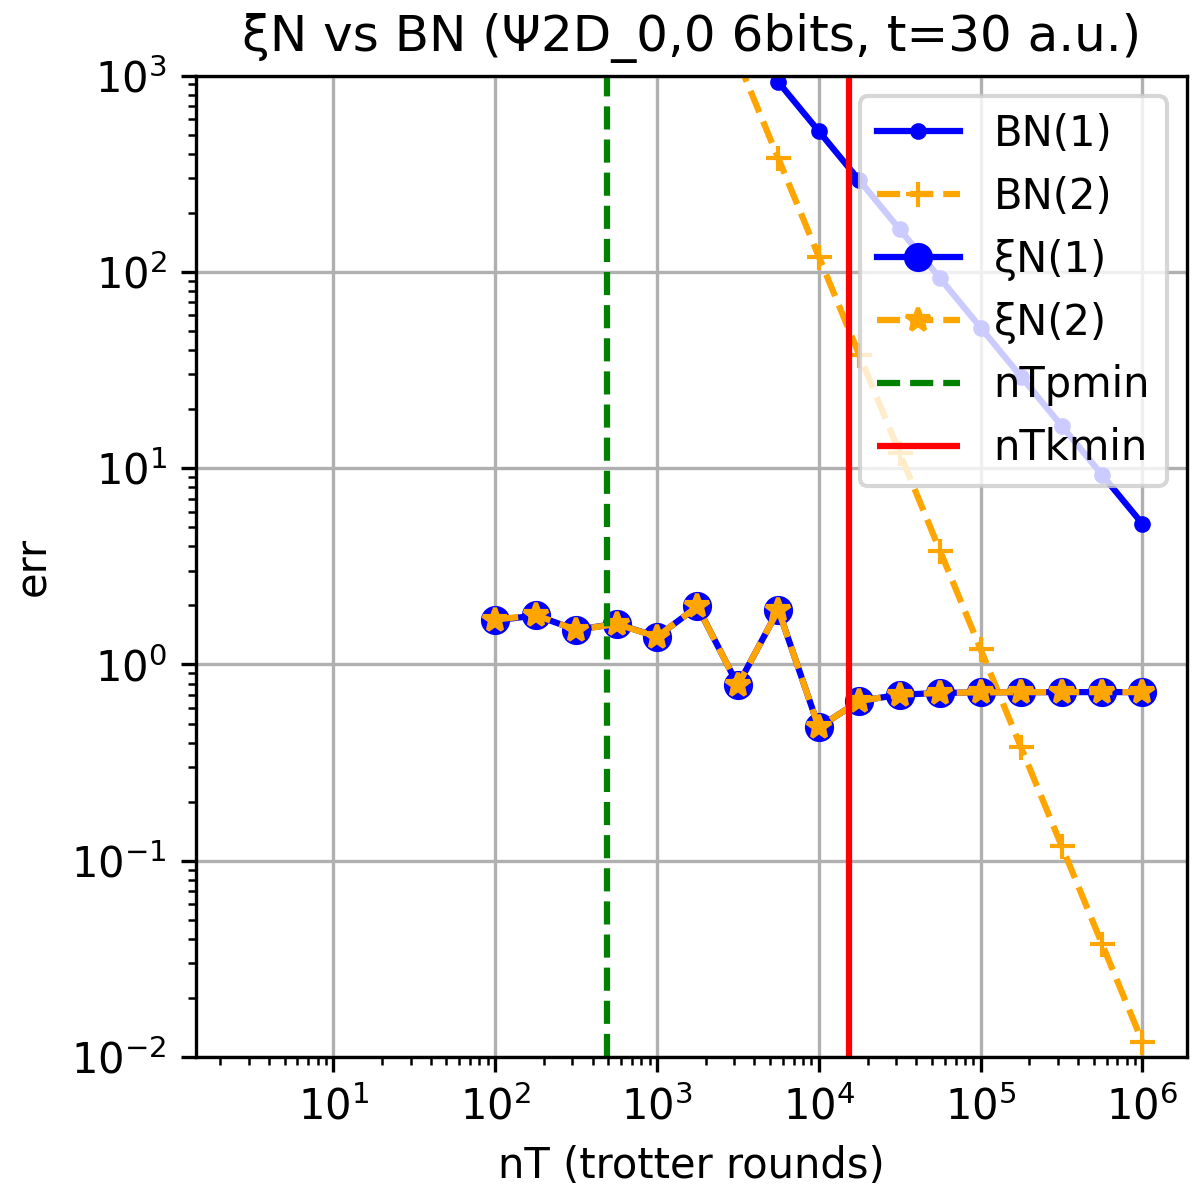
\includegraphics[width=1\columnwidth]{paper2025_figs/sdt_error/trotter_err_n0_m0_6b_t30.png}
        \caption{$\PsiTwoD_{0,0}, \nb=6, t=30.0$}
        \label{subfig:trotter-error-2d-0-0-6b-t30}
    \end{subfigure}
    \begin{subfigure}{0.45\columnwidth}
        \centering
        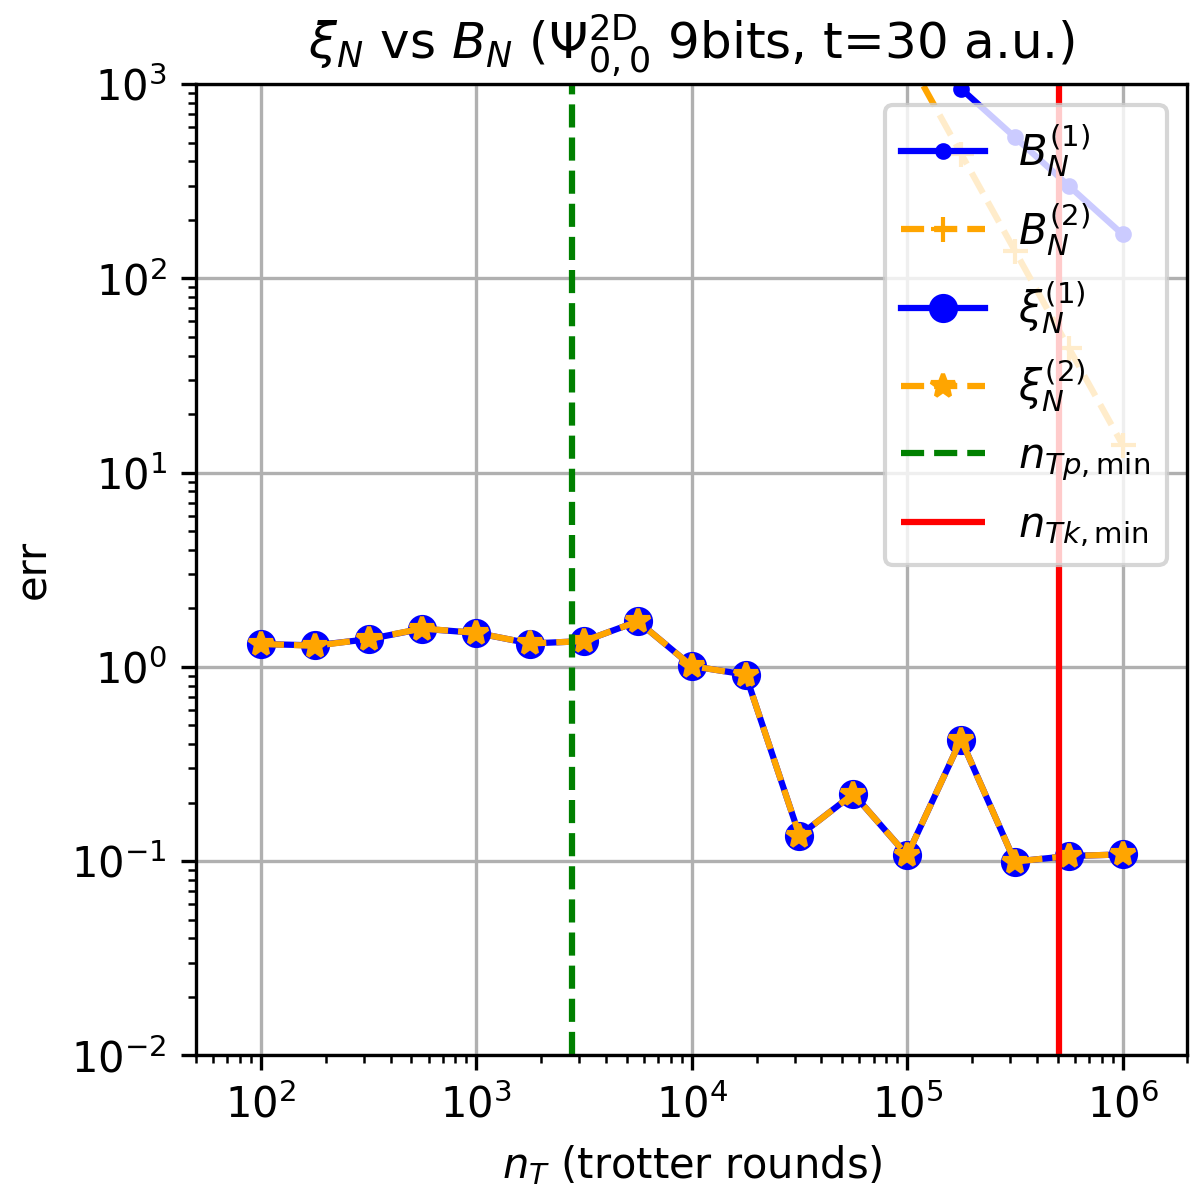
\includegraphics[width=1\columnwidth]{paper2025_figs/sdt_error/trotter_err_n0_m0_9b_t30.png}
        \caption{$\PsiTwoD_{0,0}, \nb=9, t=30.0$}
        \label{subfig:trotter-error-2d-0-0-9b-t30}
    \end{subfigure}

    \begin{subfigure}{0.45\columnwidth}
        \centering
        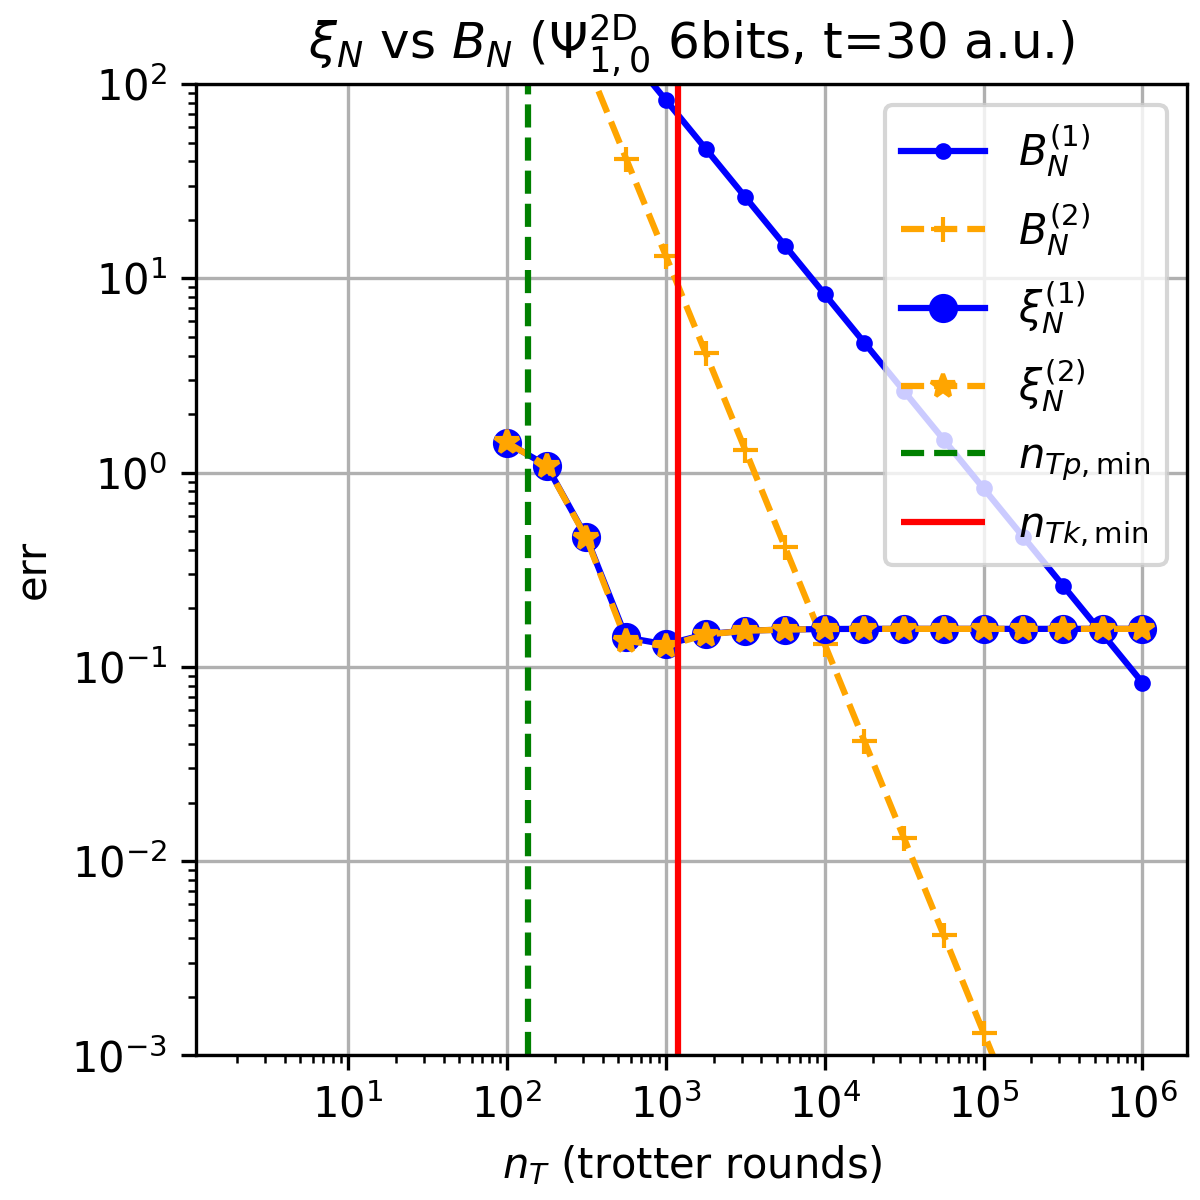
\includegraphics[width=1\columnwidth]{paper2025_figs/sdt_error/trotter_err_n1_m0_6b_t30.png}
        \caption{$\PsiTwoD_{1,0}, \nb=6, t=30.0$}
        \label{subfig:trotter-error-2d-1-0-6b-t30}
    \end{subfigure}
    \begin{subfigure}{0.45\columnwidth}
        \centering
        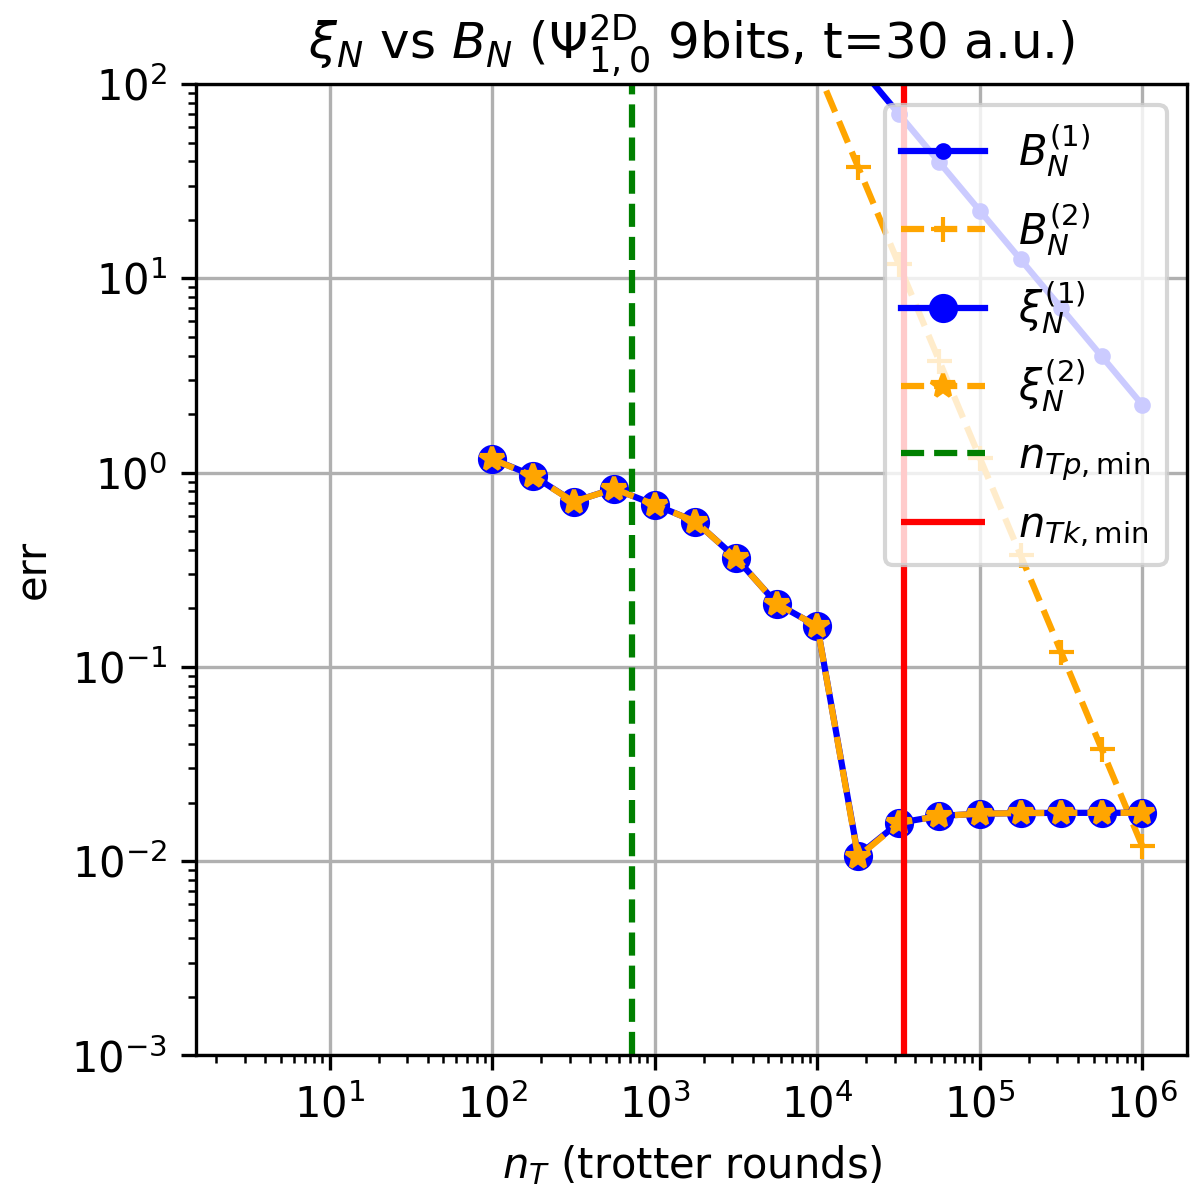
\includegraphics[width=1\columnwidth]{paper2025_figs/sdt_error/trotter_err_n1_m0_9b_t30.png}
        \caption{$\PsiTwoD_{1,0}, \nb=9, t=30.0$}
        \label{subfig:trotter-error-2d-1-0-9b-t30}
    \end{subfigure}

    \caption{Upper bound $\BN{\gamma}$ and observed value $\xiN{\gamma}$ of the error with respect to the number of divisions $\nT$ at time evolution period $t=30.0$}
    \label{fig:trotter-error-t30-part1}
\end{figure}

\begin{figure}[ht]
    \centering
    \begin{subfigure}{0.45\columnwidth}
        \centering
        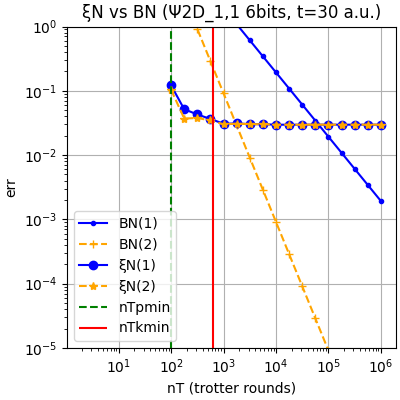
\includegraphics[width=1\columnwidth]{paper2025_figs/sdt_error/trotter_err_n1_m1_6b_t30.png}
        \caption{$\PsiTwoD_{1,1}, \nb=6, t=30.0$}
        \label{subfig:trotter-error-2d-1-1-6b-t30}
    \end{subfigure}
    \begin{subfigure}{0.45\columnwidth}
        \centering
        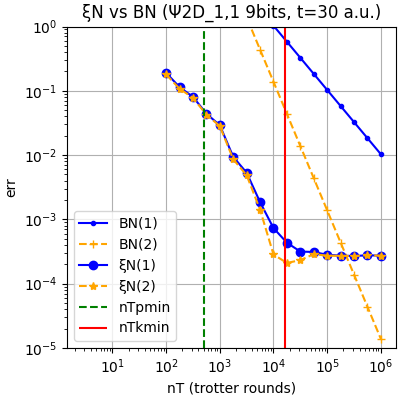
\includegraphics[width=1\columnwidth]{paper2025_figs/sdt_error/trotter_err_n1_m1_9b_t30.png}
        \caption{$\PsiTwoD_{1,1}, \nb=9, t=30.0$}  
        \label{subfig:trotter-error-2d-1-1-9b-t30}
    \end{subfigure}

    \caption{Upper bound $\BN{\gamma}$ and observed value $\xiN{\gamma}$ of the error with respect to the number of divisions $\nT$ at time evolution period $t=30.0$ (continued)}
    \label{fig:trotter-error-t30-part2}
\end{figure}

\end{document}
